% flashcards-title: Graph of total mass against number of coins
% flashcards-desc: A graph whose horizontal axis is labeled number of coins, marked from zero to ten with labels every two, and whose vertical axis is labeled total mass in grams, with labels every ten grams and small unlabeled divisions between them. Five filled dots rise from lower left to upper right. One dot is circled, with muted dashed guide lines running from the circle down to the horizontal axis and across to the vertical axis.
\documentclass[dvisvgm,tikz,border=8pt]{standalone}
\usepackage{tikz}
\usetikzlibrary{arrows.meta,calc,positioning}
\definecolor{DeckInk}{HTML}{172A3A}
\definecolor{DeckAccent}{HTML}{176B87}
\definecolor{DeckWarm}{HTML}{D97706}
\definecolor{DeckMuted}{HTML}{667784}
\definecolor{DeckPaper}{HTML}{F7FAFC}
\tikzset{
  every node/.style={font=\sffamily, text=DeckInk},
  object/.style={draw=DeckInk, line width=1.1pt, fill=DeckPaper},
  primary/.style={draw=DeckAccent, line width=1.5pt},
  boundary/.style={draw=DeckAccent, line width=1.5pt, dashed, rounded corners=6pt},
  guide/.style={draw=DeckMuted, line width=0.9pt, dashed},
  dimension/.style={{Stealth[length=3.2mm,width=2.2mm]}-{Stealth[length=3.2mm,width=2.2mm]}, draw=DeckWarm, line width=1.2pt},
  motion/.style={-{Stealth[length=3.5mm,width=2.5mm]}, draw=DeckAccent, line width=1.5pt, dashed},
}

\begin{document}
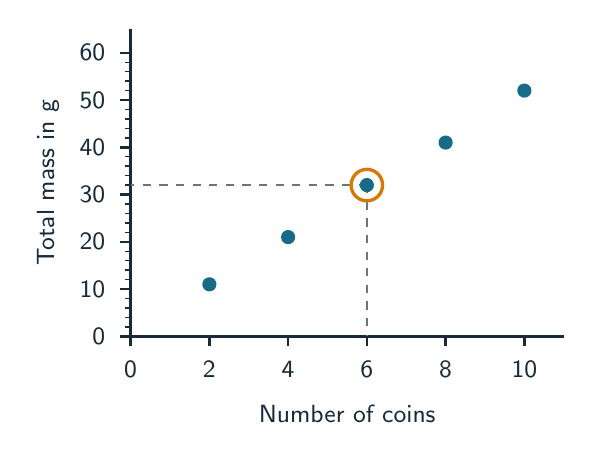
\begin{tikzpicture}[x=1cm,y=1cm]
  % x = coins * 0.5, y = grams * 0.06
  \draw[DeckInk, line width=1.1pt] (0,0) -- (5.5,0);
  \draw[DeckInk, line width=1.1pt] (0,0) -- (0,3.9);
  \foreach \x/\v in {0/0,1/2,2/4,3/6,4/8,5/10}{
    \draw[DeckInk, line width=0.9pt] (\x,0) -- (\x,-0.12);
    \node[font=\sffamily\small] at (\x,-0.42) {\v};
  }
  \foreach \y in {0.12,0.24,...,3.61}
    \draw[DeckInk, line width=0.5pt] (0,\y) -- (-0.07,\y);
  \foreach \y/\v in {0/0,0.6/10,1.2/20,1.8/30,2.4/40,3.0/50,3.6/60}{
    \draw[DeckInk, line width=0.9pt] (0,\y) -- (-0.14,\y);
    \node[font=\sffamily\small, anchor=east] at (-0.2,\y) {\v};
  }
  \node[font=\sffamily\small] at (2.75,-0.98) {Number of coins};
  \node[font=\sffamily\small, rotate=90] at (-1.05,1.95) {Total mass in g};
  \draw[guide] (3.0,1.92) -- (3.0,0);
  \draw[guide] (3.0,1.92) -- (0,1.92);
  \fill[DeckAccent] (1.0,0.66) circle (0.09);
  \fill[DeckAccent] (2.0,1.26) circle (0.09);
  \fill[DeckAccent] (3.0,1.92) circle (0.09);
  \fill[DeckAccent] (4.0,2.46) circle (0.09);
  \fill[DeckAccent] (5.0,3.12) circle (0.09);
  \draw[DeckWarm, line width=1.2pt] (3.0,1.92) circle (0.2);
\end{tikzpicture}
\end{document}
